\hypertarget{geld}{%
\chapter{Geld}\label{geld}}

\begin{blockquotebox}
    De waarde van geld wordt bepaald door de koopkracht. Het is niet de hoeveelheid geld of het gewicht ervan dat mensen willen bezitten, maar de koopkracht die het vertegenwoordigt. De marktwerking zorgt ervoor dat de koopkracht van geld zich aanpast tot een niveau waar vraag en aanbod in evenwicht zijn, waardoor er nooit te veel of te weinig geld kan zijn.\footnotemark
    \par\raggedleft--- Ludwig von Mises\index{Ludwig von Mises}
\end{blockquotebox}
\autocite{109}

\vspace{-2em}
\hypertarget{het-probleem-dat-geld-oplost}{%
\section{Het probleem dat geld oplost}\label{het-probleem-dat-geld-oplost}}

Mensen die baat hebben bij handel hebben een stimulans om meer handel te drijven. Maar de belangrijkste belemmering voor groei van de handel tussen mensen is het probleem van het niet-samenvallen van behoeften\index{samenvallen van behoeften}. Wanneer mensen oplossingen proberen te vinden voor dit probleem, leiden hun acties op natuurlijke wijze tot het ontstaan van geld, dat gedefinieerd wordt als een algemeen ruilmiddel\index{ruilmiddel}. Door te begrijpen hoe het probleem van het samenvallen van behoeften\index{samenvallen van behoeften} door geld wordt opgelost, kunnen we de karakteristieken onderscheiden die belangrijk zijn voor het succesvol functioneren van geld, en als gevolg daarvan ook de eigenschappen begrijpen die er voor zorgen dat goed geld vrij op de markt kan verschijnen.

In grote families of kleine stammen is handel waarschijnlijk ongecompliceerd en direct. Dit komt doordat iedereen elkaar kent, de mate van specialisatie in productie\index{productie} erg laag is en er een klein aantal goederen en diensten beschikbaar is. In zo\textquotesingle n primitieve omgeving is er niet veel behoefte aan het ontstaan van geld. Omdat er maar een paar goederen beschikbaar zijn, kunnen individuen deze goederen direct met elkaar verhandelen. De jager kan simpelweg zijn extra konijnen inruilen voor vis van de visser, tegen een wisselkoers\index{wisselkoers} die de twee aanvaardbaar vinden, in een transactie die \textbf{ruilhandel\index{ruilhandel}} wordt genoemd. Omdat er sterke banden tussen een kleine groep mensen bestaat, hoeven ze niet per se direct hun goederen te leveren voor onmiddellijke ruil\index{ruil}; het is mogelijk om een goed nu te ruilen voor een belofte van een goed in de toekomst. De jager kan een boer vandaag konijnen geven in ruil\index{ruil} voor een deel van de graanoogst van de boer in het oogstseizoen over een paar maanden. Als je vandaag een goed ontvangt en deze in de toekomst belooft terug te betalen, ga je een \textbf{schuld aan}.

Ruilhandel en schuld zijn twee manieren om handel te drijven, maar ze zijn alleen praktisch in specifieke en steeds minder vaak voorkomende omstandigheden. Ruilen komt voor in het zeldzame geval waarin iemand een goed wil ruilen voor een ander goed waarvan die eigenaar het eerstgenoemde goed wil hebben. Dit wordt het \textbf{samenvallen van behoeften\index{samenvallen van behoeften}} genoemd: beide partijen van de transactie willen precies wat de andere partij te bieden heeft. De visser moet een jager vinden die op zoek is naar vis, en de jager moet een visser vinden die op zoek is naar konijnen. Als konijnen en vis de enige goederen in deze economie zijn, is de kans veel groter dat ze elkaar vinden dan wanneer er miljoenen andere goederen en diensten zijn, zoals het geval is in een moderne economie. Hoe meer mensen in een samenleving en hoe groter het aantal mogelijke goederen en producten, hoe kleiner de kans dat deze twee mensen elkaar vinden om handel te drijven. In een economie met slechts 100 mensen en 10 goederen in totaal, zal iedereen betrokken zijn bij de productie\index{productie} van een van deze goederen en zal iedereen een voorraad van deze goederen hebben. De kans dat je een handelspartner vindt wiens wensen overeenkomen met die van jou neemt drastisch af naarmate het aantal mensen in een economie en het aantal beschikbare goederen en diensten toeneemt.

In de moderne wereld, waarin een grote verscheidenheid aan goederen en diensten bestaat, is ruilhandel\index{ruilhandel} praktisch onmogelijk. Familieleden en vrienden kunnen door hun nauwe relatie wel eens de kans vinden om aan ruilhandel\index{ruilhandel} te doen, maar niemand die bij zijn volle verstand is, zal op een dag wakker worden en bedenken hoe hij een manier kan vinden om goederen en diensten direct voor elkaar te ruilen. De kosten van deze zoektocht zullen waarschijnlijk hoger zijn dan de voordelen van de ruil\index{ruil}. Geen enkele groep die groter is dan een kleine stam met heel weinig goederen kan ooit een economie hebben die gebaseerd is op ruilhandel\index{ruilhandel}.

Dezelfde analyse geldt voor het gebruik van schuld als ruilmiddel\index{ruilmiddel}. In een kleine samenleving waarin individuen sterke banden hebben en afhankelijk zijn van herhaalde interactie met elkaar om te overleven, is het mogelijk om schuld te gebruiken om handel te vergemakkelijken. Maar naarmate de samenleving groter wordt en interacties plaatsvinden tussen vreemden die hoogstwaarschijnlijk geen herhaalde interacties met elkaar zullen hebben, wordt het aangaan van schuld onwerkbaar. Naarmate een economie groeit, wordt het riskanter om een handelspartner te vertrouwen. Er is geen goede reden om een belofte van betaling te accepteren van een vreemdeling, omdat er geen goede reden is om aan te nemen dat die vreemdeling waarde hecht aan zijn reputatie bij iemand die hij misschien nooit meer zal ontmoeten.

Naarmate er meer individuen in een economie zijn en het aantal goederen toeneemt, wordt het probleem van niet-samenvallende behoeften groter. Het menselijk verstand kan een oplossing voor het probleem vinden door aan \textbf{indirecte ruil\index{indirecte ruil}} te doen: goederen verkopen voor een goed waarvan het enige doel is om het weer te ruilen voor het gewenste goed. Bij indirecte ruil\index{indirecte ruil} verwerft een individu een goed niet omdat ze het wil hebben, maar omdat ze het wil ruilen voor iets anders dat ze wel wil hebben. Als de visser ontdekt dat een jager met een konijn dat hij wil hebben niet geïnteresseerd is in vis maar op zoek is naar graan, kan de visser zijn vis ruilen voor graan en het graan aan de jager geven in ruil\index{ruil} voor konijnen. Graan is voor de visser geen consumptiegoed\index{consumptiegoed}, het is een \textbf{ruilmiddel\index{ruilmiddel}}: het is een goed dat niet wordt verworven omwille van zijn eigen nut, maar om het te ruilen voor het goed dat de eigenaar werkelijk wenst.

Het vermogen van de mens om te redeneren maakt het onvermijdelijk dat deze indirecte ruiltransacties zouden ontstaan om het probleem van niet-samenvallende behoeften op te lossen. Menselijk handelen heeft echter gevolgen die verder liggen dan het bereiken van directe doelstellingen. Naarmate de marktomvang toeneemt en mensen steeds meer hun toevlucht nemen tot indirecte ruil\index{indirecte ruil}, is het logisch dat sommige goederen die functie beter vervullen dan andere, met belangrijke gevolgen voor de betrokken partijen. ``Verkoopbaarheid'' is de term die Carl Menger\index{Carl Menger} gaf aan de eigenschap die geld aantrekkelijk maakt, en hoe beter verkoopbaar een goed is, hoe succesvoller het is als geld. Als we de functie van ruilmiddelen begrijpen, kunnen we de eigenschappen begrijpen die een bepaald type geld aantrekkelijk maken.

\hypertarget{verkoopbaarheid}{%
\section{Verkoopbaarheid}\label{verkoopbaarheid}}

Menger definieert \textbf{verkoopbaarheid\index{verkoopbaarheid}} als het gemak waarmee een goed op een markt op elk geschikt moment tegen de gangbare prijzen verkocht kan worden. Hoe beter de verkoopbaarheid\index{verkoopbaarheid} van een goed is, hoe groter de kans dat de eigenaar een gangbare marktprijs, zonder te veel korting, voor zijn goed krijgt wanneer hij het wil verkopen. Een goed met een lage verkoopbaarheid\index{verkoopbaarheid} is een goed waarvan de eigenaar een aanzienlijke prijsreductie zou verwachten als hij het snel zou willen verkopen. Een goed met een hoge verkoopbaarheid\index{verkoopbaarheid} is een goed met een aanzienlijke marktdiepte en liquiditeit\index{liquiditeit}, waardoor de eigenaar de gangbare marktprijs kan krijgen wanneer hij het goed wil verkopen.

Een goed voorbeeld van een zeer verkoopbaar goed is tegenwoordig het honderd-dollarbiljet, dat wereldwijd vaker wordt geaccepteerd door winkeliers en wisselkantoren dan enig ander fysiek monetair middel. De eigenaar van een honderd-dollarbiljet die het wil inwisselen voor goederen en diensten zal het zelden hoeven te verkopen voor iets anders om dat vervolgens te geven aan een verkoper met wie hij een transactie aangaat, noch zal iemand met een honderd-dollarbiljet het ooit met korting moeten verkopen. De eigenaar vindt meestal wel iemand die het snel en tegen nominale waarde van hem overneemt. Een goed met een lage verkoopbaarheid\index{verkoopbaarheid} is daarentegen een goed waarnaar de vraag op de markt onregelmatig en gevarieerd is, waardoor het moeilijk is om het goed snel te verkopen, waardoor de eigenaar een korting moet geven om het snel te kunnen verkopen. Een goed voorbeeld hiervan is een huis, auto of andere duurzame consumptiegoederen\index{consumptiegoed}. Een huis verkopen is veel moeilijker dan een biljet van honderd dollar, omdat het bezichtigingen en aanzienlijke transactiekosten met zich meebrengt, evenals het wachten op de juiste koper die het huis waardeert tegen de vraagprijs van de verkoper. De verkoper moet misschien een aanzienlijke korting bieden om het huis snel te verkopen. Op de kapitaalmarkten zijn de meest verkoopbare instrumenten Amerikaanse staatsobligaties, die op het moment van schrijven samen ongeveer \$28.000 miljard waard zijn. De meeste grote en institutionele beleggers gebruiken Amerikaanse staatsobligaties als spaarmiddel\index{spaarmiddel} en kasreserve omdat het gemakkelijk is om grote hoeveelheden te liquideren zonder grote bewegingen in de markt te veroorzaken.

Centraal in Mengers analyse van verkoopbaarheid\index{verkoopbaarheid} is de maatstaf voor de spread tussen de bied- en laatprijs van activa. De biedprijs is de maximumprijs die een koper bereid is te betalen en de laatprijs is de minimumprijs die een verkoper accepteert als betaling. Door grote hoeveelheden van een goed op de markt te brengen wordt de spread tussen de bied- en laatprijs groter omdat, naarmate het marginale nut van het goed afneemt bij grotere hoeveelheden, potentiële kopers lagere prijzen gaan bieden. Hoe meer het marginale nut van een goed afneemt bij toenemende hoeveelheden, hoe minder het geschikt is voor de rol van geld. Hoe kleiner de afname van het marginale nut van een goed, hoe minder de bied-laat spread zal toenemen naarmate er grotere hoeveelheden op de markt komen, hoe beter het goed verkoopbaar is en hoe geschikter het is om als geld te dienen.

We kunnen dit proces ook begrijpen vanuit het perspectief van winkeliers en kooplieden die goederen kopen om later te verkopen. Voor hen verkleint een groeiende voorraad van een goed de kans dat elk marginaal goed wordt verkocht en vergroot het het risico\index{risico} van prijsdalingen ten nadele van de verkoper. Daarom zullen ze minder bieden voor steeds grotere hoeveelheden van een goed. Hoe sneller de spread tussen vraag en aanbod groeit, hoe minder verkoopbaar het goed is. Goederen waarvoor de spread langzaam stijgt, zijn beter verkoopbaar en deze goederen zullen eerder worden opgepot door iedereen die welvaart door de tijd of over een afstand wil verplaatsen. Met andere woorden, de meest verkoopbare goederen zullen het minst fluctueren in verhouding tot de hoeveelheid die op een bepaalde markt wordt gebracht.

Veel factoren, die hieronder worden besproken, kunnen de verkoopbaarheid\index{verkoopbaarheid} van goederen beïnvloeden. Dit resulteert in uiteenlopende maten van verkoopbaarheid\index{verkoopbaarheid}. De goederen met de hoogste verkoopbaarheid\index{verkoopbaarheid} zijn de goederen waarvan het marginale nut het minst afneemt met toenemende voorraden, omdat toenemende voorraden gemakkelijk kunnen worden geruild tegen andere goederen. Menger definieert geld als het meest verkoopbare goed. Tijdens het natuurlijke verloop van markttransacties zal blijken dat sommige goederen een lager afnemend marginaal nut\index{marginaal nut} en een hogere verkoopbaarheid\index{verkoopbaarheid} hebben dan andere goederen, waardoor mensen worden aangemoedigd er meer van aan aan te houden, wat leidt tot een grotere liquiditeit\index{liquiditeit} van het goed en een verdere toename van de verkoopbaarheid\index{verkoopbaarheid}. Dit proces zal op natuurlijke wijze de verkoopbaarheid\index{verkoopbaarheid} van de meest verkoopbare goederen vergroten, waardoor de monetaire rol geconcentreerd wordt in de meest verkoopbare goederen. Uiteindelijk zal deze monetaire rol zich concentreren in slechts één goed, het meest verkoopbare goed, het algemene ruilmiddel\index{ruilmiddel}: geld, het goed waarvan het marginale nut het minst afneemt.

Het onderstaande numerieke voorbeeld kan ons helpen om de verkoopbaarheid\index{verkoopbaarheid} van geld te begrijpen. Voor het gemak nemen we aan dat de marktprijs van elke appel, sinaasappel en banaan gelijk is aan één monetaire eenheid, en we drukken het nut uit in kardinale termen. Daarbij moeten we wel inzien dat mensen nut alleen begrijpen in ordinale termen, zoals hierboven al is besproken.

\begin{table}[!htb]
\centering
\begin{tabular}{|c|c|c|c|c|}  % Add vertical lines
\hline  % Top horizontal line
    \cellcolor{gray!25} Goed &
    \cellcolor{gray!25} Appel &
    \cellcolor{gray!25} Sinaasappel &
    \cellcolor{gray!25} Banaan &
    \cellcolor{gray!25} Geld \\
\hline  % Horizontal line after the header
 %
 Nut van de 1\textsuperscript{e} eenheid & 100 & 90 & 85 & 100 (1\textsuperscript{e} appel) \\ \hline
 Nut van de 2\textsuperscript{e} eenheid & 80 & 70 & 65 & 90 (1\textsuperscript{e} sinaasappel) \\ \hline
 Nut van de 3\textsuperscript{e} eenheid & 60 & 50 & 45 & 85 (1\textsuperscript{e} banaan) \\ \hline
 Nut van de 4\textsuperscript{e} eenheid & 40 & 30 & 25 & 80 (2\textsuperscript{e} appel) \\ \hline
 Nut van de 5\textsuperscript{e} eenheid & 20 & 10 & 5 & 70 (2\textsuperscript{e} sinaasappel) \\ \hline
 Nut van de 6\textsuperscript{e} eenheid & 0 & 0 & 0 & 65 (2\textsuperscript{e} banaan) \\ \hline  % Bottom horizontal line
\end{tabular}
\caption{Het afnemende nut van geld}
\label{tab1}
\end{table}



Naarmate het marginale nut van elk goed afneemt, neemt het marginale nut van de monetaire eenheden minder af dan het nut van het goed. Omdat geld het meest verkoopbare goed is, is het het gemakkelijkst in te ruilen voor consumptiegoederen\index{consumptiegoed} en daarom meer geaccepteerd als betaalmiddel. Voor deze persoon is het accepteren van geld een betere optie dan het accepteren van appels, sinaasappels of bananen, omdat het geld gemakkelijk inwisselbaar is voor welk van deze consumptiegoederen\index{consumptiegoed} de persoon op een toekomstig tijdstip dan ook het meest zal waarderen. Sommige economische goederen zijn geschikter om de rol van ruilmiddel\index{ruilmiddel} te vervullen dan andere. Hoe geschikter een goed is om te gebruiken voor ruil\index{ruil}, hoe beter verhandelbaar of verkoopbaar het is.

Door te begrijpen welk probleem geld oplost, kunnen we beter vaststellen welke eigenschappen een goede oplossing moet hebben --- met andere woorden, ze helpt ons te bepalen wat iets tot goed geld maakt. Het probleem dat geld oplost, is het gebrek aan samenvallen van behoeften\index{samenvallen van behoeften}, en het manifesteert zich in verschillende dimensies. Er is het gebrek aan samenvallen van behoeften\index{samenvallen van behoeften} in de goederen zelf, zoals besproken in het voorbeeld van vis, konijnen en graan hierboven. Daarnaast is er het gebrek aan het samenvallen van behoeften\index{samenvallen van behoeften} over afstand. Dat wil zeggen, iemand kan iets willen verkopen op de ene locatie en er een goed voor krijgen op een andere locatie. Je appels ruilen voor een auto zou in de meeste scenario\textquotesingle s al moeilijk genoeg zijn, maar het zou nog moeilijker zijn als je je appels 1.000 kilometer zou moeten sjouwen om de transactie uit te voeren.

De derde dimensie van het samenvallen van behoeften\index{samenvallen van behoeften}, is het gebrek aan het samenvallen van behoeften\index{samenvallen van behoeften} op schaal. Wanneer individuen goederen van verschillende grootte en waarde rechtstreeks willen ruilen, is een gedeeltelijke ruil\index{ruil} niet altijd mogelijk. De persoon die appels wil verkopen, kan niet elke appel ruilen voor een onderdeel van een auto van iemand anders en vervolgens de onderdelen samenvoegen tot één auto. Het zou onpraktisch en inefficiënt zijn om handel te drijven met zulke verschillende goederen. Ons menselijk verstand suggereert dat een ander, beter deelbaar ruilmiddel\index{ruilmiddel} het probleem zal oplossen.

Naast de dimensies van het goed, de afstand en de schaal, is er nog een vierde dimensie aan het probleem van samenvallen van behoeften\index{samenvallen van behoeften}: het gebrek aan samenvallen van het tijdsbestek voor de handel. Iemand kan een voorwerp vandaag willen verkopen of over een bepaalde periode, om in de toekomst een ander goed te verkrijgen. Iemand wil misschien gedurende een periode van drie jaar appels verkopen om zo een auto te kunnen kopen. Het is niet mogelijk om voor drie jaar aan appels te verzamelen en dit om te ruilen voor een auto, omdat de appels zullen bederven. Het menselijk verstand brengt hem er natuurlijk toe het gemak in te zien van het ruilen van appels voor een ruilmiddel\index{ruilmiddel} -- een ruilmiddel\index{ruilmiddel} dat niet zal rotten of door wormen zal worden opgegeten -- waarmee hij in de toekomst een auto kan kopen.

Door de verschillende assen te onderzoeken waarlangs het probleem van het samenvallen van behoeften\index{samenvallen van behoeften} zich voordoet, wordt het mogelijk om de eigenschappen te identificeren die een goed ruilmiddel\index{ruilmiddel} vormen. De eigenschappen die iets tot een goed ruilmiddel\index{ruilmiddel} maken, maken het tot een goede oplossing voor het probleem van het samenvallen van behoeften\index{samenvallen van behoeften} in zijn vier dimensies. Zoals Murray Rothbard\index{Murray Rothbard} het stelde: ``De vraag naar gebruik door meer mensen, de deelbaarheid in kleinere eenheden zonder waardeverlies, de duurzaamheid en de mogelijkheid om over grote afstanden te worden vervoerd, dragen allemaal bij aan de verkoopbaarheid\index{verkoopbaarheid} van een goed.''\autocite{110}

\begin{table}[!htb]
\centering
\begin{tabular}{| p{1.2cm} | p{4.2cm} | p{4.2cm} |}
\hline
 & \textbf{Beschrijving van het probleem} & \textbf{Hoe geld dit oplost} \\ \hline
\textit{Goederen} & Ik wil een goed kopen waarvan de verkoper niet wil wat ik heb & Focus op het kleinst mogelijke aantal middelen \\ \hline
\textit{Ruimte} & Ik wil iets verkopen op een plaats en iets anders kopen op een andere plaats & Vervoerbaar \\ \hline
\textit{Schaal} & Ik wil iets groots verkopen en iets kleins kopen & Homogeen, deelbaar en samenstelbaar \\ \hline
\textit{Tijd} & Ik wil vandaag iets verkopen om in de toekomst iets te kunnen kopen & Duurzaam, moeilijk te produceren \\ \hline
\end{tabular}
\caption{Dimensies van het probleem van het samenvallen van behoeften\index{samenvallen van behoeften}}
\end{table}\label{tab2}


Het derde facet van het probleem van het samenvallen van behoeften\index{samenvallen van behoeften} helpt ons te begrijpen waarom metalen van nature een betere keuze waren als monetair middel dan artefacten en andere consumptiegoederen\index{consumptiegoed}. Omdat metalen bestaan uit een homogene substantie, kunnen grote hoeveelheden metaal worden opgedeeld in kleinere coupures, terwijl kleine hoeveelheden kunnen worden samengevoegd tot grotere stukken zonder significant verlies van economische waarde of een verandering in de fysieke eigenschappen van het metaal. Metaal is dus zeer deelbaar en makkelijk weer samen te voegen. Dat is geen eigenschap van artefacten zoals schelpen, vee en glazen kralen.

Het tweede facet van het probleem van het samenvallen van behoeften\index{samenvallen van behoeften}, de verkoopbaarheid\index{verkoopbaarheid} over afstand, helpt ons te begrijpen waarom goud\index{goud} en zilver\index{zilver} van oudsher geschikt waren voor hun monetaire rol, evenals de moderne beperkingen die deze metalen vandaag de dag verhinderen deze rol te spelen. Door hun inertheid, rotten, verweren, roesten of bederven zilver\index{zilver} en goud\index{goud} niet. Deze metalen kunnen relatief gemakkelijk worden verplaatst, met weinig zorgen dat het transport hun eigenschappen zal veranderen of hun integriteit zal aantasten. Omdat ze grote hoeveelheden economische waarde in kleine gewichten concentreren, zijn deze metalen bijzonder voordelig om te verplaatsen in vergelijking met andere monetaire middelen. Maar toen de moderne telecommunicatie- en transportindustrieën geavanceerder werden met de komst van de Industriële Revolutie in de negentiende eeuw, raakte de wereld veel meer onderling verbonden en begon de omvang van de wereldhandel zich uit te breiden. Door de toenemend wereldwijde handel en de handel over lange afstanden was het verplaatsen van fysiek goud\index{goud} en zilver\index{zilver} niet langer een economisch\index{economisch} verantwoorde methode om handel te drijven. Krediet op basis van deze metalen werd een volwaardig ruilmiddel\index{ruilmiddel} en uiteindelijk zorgde de overname van bankinstellingen door de overheid\index{overheid} ervoor dat overheidskrediet goud\index{goud} en zilver\index{zilver} in de Eerste Wereldoorlog\index{Eerste Wereldoorlog} effectief kon verdringen.\footnote{Zoals meer in detail wordt besproken in \emph{De Fiat Standaard}.}

Historisch gezien hadden zilver\index{zilver} en goud\index{goud} een dubbele monetaire rol, omdat ze elkaar aanvulden wat betreft verkoopbaarheid\index{verkoopbaarheid} op verschillende niveaus. Goud, dat waardevoller was, was moeilijk te verdelen in hele kleine stukjes voor transacties van kleine waarde, terwijl zilver\index{zilver}, dat minder waardevol was, niet erg geschikt was voor grote transacties. Historisch gezien was ook koper een geschikt monetair middel voor kleinere waarde-eenheden dan zilver\index{zilver}. Na verloop van tijd verloren koper en zilver\index{zilver} hun monetaire rol om redenen die te maken hadden met verkoopbaarheid\index{verkoopbaarheid} door tijd, zoals hieronder wordt besproken. Met de globalisering van markten\index{markten} en de ongekende omvang van internationale handel aan het einde van de negentiende eeuw, koos de wereldeconomie voor één geldsoort, goud\index{goud}, als oplossing voor het probleem van het samenvallen van behoeften\index{samenvallen van behoeften}.

\hypertarget{verkoopbaarheid-door-tijd}{%
\section{Verkoopbaarheid door tijd}\label{verkoopbaarheid-door-tijd}}

Het vierde facet van het probleem van het samenvallen van wensen heeft betrekking op de mogelijkheid om waarde uit te wisselen in de tijd. Om waarde door tijd te behouden of uit te wisselen is er een ruilmiddel\index{ruilmiddel} nodig dat zijn waarde door tijd kan behouden zonder al te veel verlies. Hoe beter een ruilmiddel\index{ruilmiddel} zijn waarde door de tijd heen kan behouden, hoe geschikter en wenselijker het is als ruilmiddel\index{ruilmiddel}. Dit helpt ons te begrijpen waarom metalen een monetaire rol spelen, omdat ze over het algemeen duurzaam zijn, en waarom edelmetalen, zoals goud\index{goud} en zilver\index{zilver} in het bijzonder, een prominentere, langdurigere monetaire rol zouden spelen dan basismetalen zoals ijzer en koper. Omdat ze inert en onverwoestbaar zijn, hebben edelmetalen een belangrijk voordeel ten opzichte van metalen die na verloop van tijd vergaan. Maar het echte voordeel van deze metalen ligt niet alleen in hun stabiliteit, maar in het effect van deze stabiliteit op de dynamiek van hun aanbod. Het belangrijkste kenmerk dat edelmetalen onderscheidt van alle andere vormen van geld is de relatieve grootte van de voorraden ten opzichte van de jaarlijkse productie\index{productie}. Omdat deze metalen niet roesten of verrotten, blijven hun voorraden in de loop van de tijd groeien en raken ze zelden uitgeput. Naarmate de technologie voortschrijdt en mensen ingenieuzere manieren vinden om het aanbod van deze metalen te vergroten, blijven de voorraden groeien en blijft de bestaande productie\index{productie} een kleine fractie van de totale beschikbare voorraden.

Deze eigenschap staat bekend als hardheid, wat de moeilijkheid om de bestaande beschikbare voorraden van een goed te vergroten inhoudt. En we kunnen hardheid kwantificeren met behulp van een eenvoudige berekening, de stock-to-flow ratio, waarin stock verwijst naar de totale bovengrondse beschikbare voorraden die gebruikt kunnen worden in een monetaire rol, terwijl flow verwijst naar de nieuwe jaarlijkse productie\index{productie} door delving. Deze berekening is simpelweg het omgekeerde van het jaarlijkse groeipercentage van het aanbod en zowel theoretische argumenten als historisch bewijs geven aan dat deze verhouding enorm belangrijk is bij het bepalen van de monetaire status. Alle metalen die kunnen corroderen worden constant verbruikt in industriële processen, die hun chemische eigenschappen veranderen en ze wegnemen uit de voorraden die worden gebruikt om waarde in op te slaan. Voor al deze metalen zijn de bestaande beschikbare voorraden van dezelfde orde van grootte als de jaarlijkse productie\index{productie} van het metaal. Er zijn zeer weinig voorraden aan koper, nikkel, messing en andere metalen die gebruikt kunnen worden als spaarmiddel\index{spaarmiddel}. Voor zover dergelijke voorraden bestaan, worden ze in reserve gehouden voor producenten die er grote hoeveelheden van gebruiken en ze nodig hebben om zich in te dekken tegen mogelijke leveringsproblemen die hun productie\index{productie} stil zouden kunnen leggen. De productie\index{productie} van deze metalen wordt constant ingezet voor industrieel gebruik, dus de voorraden nemen niet significant toe. De nieuwe productie\index{productie} is dus aanzienlijk in vergelijking met de bestaande voorraden, wat de prijs\index{prijs} van het metaal erg kwetsbaar maakt voor aanbodschokken. Zulke metalen zijn ongeschikt om een monetaire rol te spelen, omdat hun verkoopbaarheid\index{verkoopbaarheid} door tijd kan worden aangetast door aanbodschokken, en hun inzet als monetair middel zal noodzakelijkerwijs aanbodschokken met zich meebrengen die hun monetaire rol tenietdoen.

Om te begrijpen waarom, moeten we eerst een onderscheid maken tussen de \textbf{marktvraag\index{marktvraag}} naar een goed, waarbij consumenten vraag uitoefenen naar het goed met als doel het te bewaren of te consumeren omwille van het goed zelf en zijn eigenschappen, en de \textbf{monetaire vraag\index{monetaire vraag}} naar een goed, waarbij consumenten het goed enkel als een monetair middel aanhouden, met het doel het later te ruilen voor andere goederen en diensten. Een persoon kan elk goed kiezen als spaarmiddel\index{spaarmiddel} en ruilmiddel\index{ruilmiddel}, en met die keuze voegt men monetaire vraag\index{monetaire vraag} toe aan de marktvraag\index{marktvraag}, wat resulteert in een stijging van de marktprijs. Dit zal natuurlijk leiden tot een toename van de hoeveelheid middelen, kapitaal\index{kapitaal} en arbeid die aan de productie\index{productie} ervan worden besteed. Dit is waar de stock-to-flow ratio van belang is. Als het goed een lage stock-to-flow ratio heeft, zal het deel van het beschikbare aanbod (stock) op de markt dat geproduceerd wordt door mijnen zeer hoog zijn, en stijgingen in gedolven productie\index{productie} (flow) zullen overeenkomen met grote stijgingen in het beschikbare aanbod op de markt, waardoor de prijs\index{prijs} daalt en de spaarders gestraft worden. De markt reageert in hoge mate op productiestijgingen van mijnen omdat de dagelijkse liquiditeit\index{liquiditeit} op de markt voornamelijk afkomstig is van nieuwe productie\index{productie} van mijnen en niet van de voorraden die consumenten aanhouden, aangezien consumenten het goed voornamelijk aanhouden om het in te zetten bij de productie\index{productie} op de markt en niet om het door te verkopen. De overwegend industriële aard van deze metalen betekent dat iedereen die ze als geld gebruikt, zijn rijkdom aan de mijnbouwbedrijven schenkt in een proces dat we zouden kunnen omschrijven als de ``val van zacht geld\index{zacht geld}''. Het opslaan van waarde in een goed met een lage stock-to-flow ratio leidt er simpelweg toe dat die waarde toevalt aan de producenten van het goed.

Om te voorkomen dat grondstoffen de \textit{easy money trap} niet kunnen weerstaan en doorheen de tijd goed verkoopbaar zullen blijven, moeten de beschikbare voorraden aanzienlijk groter zijn dan de jaarlijkse productie\index{productie}, zodat wanneer de monetaire vraag\index{monetaire vraag} stijgt, stijgingen in de productie\index{productie} weinig invloed zullen hebben op de marktomstandigheden, aangezien de mijnbouwproductie slechts een kleine fractie is van het beschikbare aanbod dat wordt verhandeld. Met een hoge stock-to-flow ratio vertalen stijgingen in de monetaire vraag\index{monetaire vraag} zich in prijsstijgingen, maar als de stock-to-flow ratio laag is, vertalen deze stijgingen zich in hogere winsten voor de mijnen.

Hard geld is geld waarvan de hoeveelheid moeilijk significant te verhogen is door producenten, ongeacht hun inspanningen, omdat de hoeveelheid die door producenten kan worden toegevoegd slechts een klein deel uitmaakt van de bestaande voorraden. Zacht geld is geld waarvan de beschikbare voorraden makkelijk te vergroten zijn. Deze term is zowel van toepassing op goederengeld als op nationale valuta. Zacht geld is in de wereld eerder regel dan uitzondering, vooral in landen die zuchten onder een slecht monetair beleid, waar de burgers heel goed de aantrekkelijkheid van relatief harde nationale valuta zoals de dollar en de euro en het gebrek aan aantrekkelijkheid van hun lokale valuta begrijpen, die de lokale overheid\index{overheid} en het kartel van centrale banken makkelijk in steeds grotere hoeveelheden kunnen produceren.

De stock-to-flow ratio ligt voor bijna alle metalen, behalve voor goud\index{goud} en zilver\index{zilver}, rond de 1. Omdat de productie\index{productie} van basismetalen voortdurend wordt verbruikt in industriële toepassingen, zijn de bestaande voorraden nooit significant hoger dan de jaarlijkse productie\index{productie}. Omdat deze metalen ook op verschillende manieren roesten en corroderen, is er weinig reden om grote hoeveelheden voor de lange termijn op te slaan. De drie belangrijkste opslagplaatsen voor op de beurs verhandelbaar koper hebben consequent samen minder dan 1.000.000 ton koper, terwijl de jaarlijkse koperproductie rond de 25.000.000 ton ligt.\autocite{111} Zelfs als de wereldwijde kopermagazijnen 20 keer meer koper zouden bevatten dan de drie belangrijkste, zou dat nog steeds niet voldoende zijn om de stock-to-flow van koper boven de 1 te brengen. In september 2020 bedroegen de zinkvoorraden op de drie belangrijkste handelsbeurzen in totaal 133.300 ton, terwijl de jaarlijkse productie\index{productie} ongeveer 13.000.000 ton bedroeg, ongeveer 100 keer meer dan de voorraad, waardoor de stock-to-flow ratio van zink 0,01 bedroeg.\autocite{112}

Omdat goud\index{goud} als metaal niet kan worden geconsumeerd of veranderd, wordt het voornamelijk verworven om aan te houden als liquide monetaire reserve. De bestaande voorraden zijn meestal vele malen groter dan de jaarlijkse productie\index{productie}. Zelfs als de jaarlijkse productie\index{productie} door meer efficiëntie toeneemt, blijven de voorraden ook toenemen, waardoor de stock-to-flow ratio aanzienlijk hoger blijft dan 1. Als we de gegevens van de afgelopen eeuw bekijken, zien we dat de stock-to-flow ratio van goud\index{goud} constant rond de 60 is gebleven, wat zich vertaalt in een jaarlijkse aanbodgroei van ongeveer 1,5\%. Zelfs als de jaarlijkse productie\index{productie} van goud\index{goud} in de loop van de tijd blijft toenemen, nemen de voorraden ook toe en blijft de verhouding ongeveer constant (Zie Figuur 6).

Zilver is met een stock-to-flow ratio hoger dan 1 vergelijkbaar met goud\index{goud}, maar historisch gezien is de stock-to-flow ratio afgenomen omdat steeds grotere hoeveelheden zilver\index{zilver} die gebruikt worden in industriële toepassingen effectief uit de beschikbare voorraden worden gehaald. Als we de stock-to-flow ratio van zilver\index{zilver} zouden meten op basis van de totale voorraad aan bovengronds zilver\index{zilver}, dan zou de stock-to-flow ratio tussen de 30 en 60 liggen.\autocite{113} Maar het zilver\index{zilver} dat gebruikt wordt in industriële toepassingen kan niet gerekend worden tot de beschikbare voorraad omdat het geen monetaire rol kan spelen, noch gebruikt kan worden om handel te drijven en schulden te vereffenen. De prijs\index{prijs} van elektronica, machines, bestek of sieraden die zilver\index{zilver} bevatten is niet afhankelijk van de monetaire prijs\index{prijs} van het zilver\index{zilver} dat het bevat, die meestal maar een klein deel van de totale prijs\index{prijs} uitmaakt, maar van de waardering die consumenten aan het goed zelf geven -- als consumptiegoed\index{consumptiegoed} of kapitaalgoed\index{kapitaalgoederen}, niet als monetair goed. Proberen het zilver\index{zilver} uit deze goederen te halen om het om te zetten in een monetair goed, in de vorm van baren of munten\index{munten}, is een kostbaar proces dat niet verschilt van het winnen van zilver\index{zilver} uit de aardkorst. Als de gebruikte maatstaf voor voorraden alleen betrekking heeft op monetaire voorraden, in de vorm van zilverbaren, munten\index{munten} en beleggingsproducten, dan ligt de stock-to-flow ratio dichter bij 4. Dit is nog steeds aanzienlijk hoger dan niet-monetaire metalen, waarvan de stock-to-flow ratio een fractie van 1 is, maar lang niet hoog genoeg om de waarde goed genoeg vast te houden om een monetaire rol te spelen. Dat is de reden waarom, terwijl de marktwaarde van zilver\index{zilver} in de afgelopen anderhalve eeuw is gedaald ten opzichte van goud\index{goud}, de niet-monetaire toepassingen zodanig zijn toegenomen dat het grootste deel van de bestaande voorraden zijn verbruikt.

Als we al het zilver\index{zilver} dat gebruikt wordt in industriële toepassingen zouden beschouwen als onderdeel van de zilvervoorraad, dan zou de stock-to-flow ratio van zilver\index{zilver} aanzienlijk hoger zijn. Echter, door de toename van het niet-monetaire gebruik van zilver\index{zilver}, is de voorraad monetair zilver\index{zilver} opgebruikt en is de stock-to-flow ratio gedaald. Tegelijkertijd is de marktwaarde van zilver\index{zilver} in reële termen gedaald.

De demonetisering van zilver\index{zilver} heeft waarschijnlijk zijn wortels in de lagere stock-to-flow ratio van het metaal en de vooruitgang van het moderne bankieren. Toen het moderne bankieren en de telecommunicatietechnologie zich in de negentiende eeuw verder ontwikkelden, konden mensen transacties uitvoeren met financiële instrumenten zoals papiergeld, cheques en kredietbrieven die gedekt werden door goud\index{goud} van banken en centrale banken. Dit maakte transacties met goud\index{goud} op elke schaal mogelijk, waardoor de monetaire rol van zilver\index{zilver}, die voornamelijk voor kleine transacties van belang was, overbodig werd en iedereen de activa kon bezitten met de hoogste stock-to-flow en de grootste kans op waardestijging.

De demonetisering van zilver\index{zilver} begon pas echt in 1871, na het einde van de Frans-Pruisische oorlog\index{oorlog}. Duitsland, dat toen de grootste economie was die nog op een zilveren standaard draaide, vroeg aan Frankrijk om zijn schadeloosstelling in goud\index{goud} uit te betalen en gebruikte deze vergoeding om over te schakelen op een goudstandaard\index{goudstandaard}. Toen de vraag van Duitsland naar zilver\index{zilver} afnam en de vraag naar goud\index{goud} toenam, begon de waarde van zilver\index{zilver} te dalen in verhouding met de goudprijs. De verhouding was ongeveer 15:1. Dit veroorzaakte economische verliezen voor zilverbezitters en landen op een zilverstandaard, wat hen aanmoedigde om hun zilver\index{zilver} in te ruilen voor goud\index{goud}. Sindsdien is de verhouding tussen de goudprijs en de zilverprijs alleen maar gestegen; momenteel ligt deze rond de 80:1, oftewel meer dan vijf keer de verhouding van 150 jaar geleden. Landen die te laat de zilverstandaard loslieten, zoals India en China, ondervonden ernstige economische problemen door de daling van de waarde van hun valuta.

\begin{figure}[!htb]
\centering
    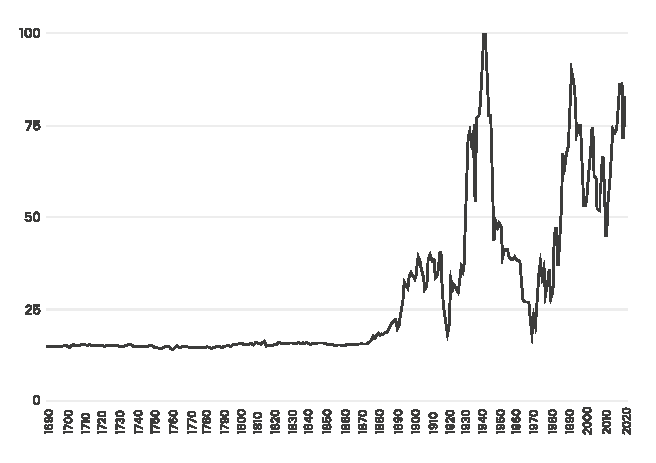
\includegraphics[width=\textwidth]{figures/fig19.pdf}
    \caption[Goud/zilver\index{zilver} verhouding]{Goud/zilver\index{zilver} verhouding}
    \label{fig19}
\end{figure}

De hoge stock-to-flow ratio van goud\index{goud} heeft ervoor gezorgd dat het een monetaire rol heeft kunnen spelen, omdat het de beste verkoopbaarheid\index{verkoopbaarheid} door de tijd heen geeft. Omdat de productie\index{productie} van goud\index{goud} slechts kleine hoeveelheden toevoegt aan de voorraad van het metaal, behoudt het zijn waarde in de loop van de tijd beter, waardoor de marktwaarde die erin is opgeslagen in de loop van de tijd toeneemt door de waardestijging ten opzichte van andere grondstoffen. Een waardestijging van tegoeden gehouden in een bepaald middel komt overeen met een toename van de liquiditeit\index{liquiditeit} van die markt, een afname van de bied-laat spread en dus een toename van de verkoopbaarheid\index{verkoopbaarheid} van de grondstof. Deze trend wordt daardoor alleen maar versterkt naarmate mensen er zich bewuster van worden en meer van hun contante geldreserves gaan aanhouden in de vorm van het goed met de hoogste verwachte toekomstige waarde en de kleinste bied-laat spread. Deze trend wordt daardoor alleen maar versterkt.

Het raamwerk van verkoopbaarheid\index{verkoopbaarheid} door tijd en de stock-to-flow ratio zijn bijzonder interessante hulpmiddelen om te gebruiken bij het analyseren van de opkomst van bitcoin\index{bitcoin}, een nieuw monetair fenomeen met een voorgeprogrammeerde aanboddynamiek en een stock-to-flow ratio die constant toeneemt tot het oneindig is. Dit analytisch kader vormt de basis van mijn eerste boek, \emph{De Bitcoin Standaard}.

\vspace{-1em}
\hypertarget{waarom-euxe9n-geldsoort}{%
\section{Waarom één geldsoort?}\label{waarom-euxe9n-geldsoort}}

Een grotere monetaire vraag\index{monetaire vraag} naar het meest verkoopbare goed zal de prijs\index{prijs} en waarde ervan verder verhogen, waardoor de verkoopbaarheid\index{verkoopbaarheid} ervan door tijd nog verder toeneemt en de liquiditeit\index{liquiditeit} ervan groeit. Aangezien rijkdom zich van nature concentreert in de meest verkoopbare goederen, zal dit de verkoopbaarheid\index{verkoopbaarheid} ervan verder vergroten. Eigenaars van de meest verkoopbare goederen zullen een grotere markt en een grotere hoeveelheid liquiditeit\index{liquiditeit} hebben waarmee ze kunnen handelen. Het toenemende gebruik als geld verhoogt de waarde van een goed als geld, waardoor de stimulans om het als geld te gebruiken toeneemt, wat resulteert in een ``winner-takes-all'' dynamiek op de geldmarkt. De geschiedenis toont aan dat dit het geval is. Aan het eind van de negentiende eeuw was de hele planeet overgeschakeld op goud\index{goud} als geld, zelfs toen duizenden verschillende goederen over de hele wereld voor deze rol werden gebruikt. Het voortbestaan van de monetaire rol van zilver\index{zilver} in de negentiende eeuw was een gevolg van de superieure verkoopbaarheid\index{verkoopbaarheid} op kleine schaal, maar toen het moderne bankieren dit overbodig maakte, werd goud\index{goud} het geld van de wereld. Iets soortgelijks gebeurt op de moderne wereldmarkt voor overheidsgeld\index{overheidsgeld}, waar er een onverzadigbare vraag lijkt te zijn naar het meest verhandelbare overheidsgeld\index{overheidsgeld}, de Amerikaanse dollar\index{Amerikaanse dollar}. Niet alleen willen heel veel niet-Amerikanen de Amerikaanse dollar\index{Amerikaanse dollar} bezitten in plaats van hun nationale valuta, vrijwel alle nationale valuta worden gedekt door dollars, omdat hun centrale banken grote hoeveelheden dollars bezitten die ze gebruiken voor de internationale handel.

Hoe algemener het ruilmiddel\index{ruilmiddel} gebruikt wordt, hoe beter het verkoopbaar is en hoe groter de potentiële markt waaraan de eigenaar kan verkopen. Individuen zullen zich van nature richten op de meest verkoopbare goederen en dat zal op zijn beurt hun verkoopbaarheid\index{verkoopbaarheid} vergroten, waardoor meer individuen worden aangetrokken om ze te gebruiken. Rothbard legde het proces als volgt uit: ``Zo gauw de meer verkoopbare goederen in een samenleving worden gekozen als ruilmiddel\index{ruilmiddel}, zullen de keuzes zich snel richten op de weinige best verkoopbare goederen die beschikbaar zijn.''\autocite{114}

Het fundamentele probleem van het samenvallen van behoeften\index{samenvallen van behoeften} betreft het samenvallen van behoeften\index{samenvallen van behoeften} naar goederen. Naarmate de omvang van een economie toeneemt, neemt ook de mate van specialisatie en het aantal goederen dat kan worden geproduceerd toe, waardoor de mogelijkheden voor directe ruilhandel\index{ruilhandel} worden bemoeilijkt. De enige mogelijke oplossing voor dit probleem, en de enige manier waarop de omvang van een markt kan groeien, is door gebruik te maken van indirecte ruil\index{indirecte ruil}, waarbij mensen goederen kopen puur om ze later te ruilen voor andere goederen. Omdat mensen verschillende goederen indirect met elkaar ruilen, is het logisch dat sommige goederen de rol van ruilmiddel\index{ruilmiddel} beter spelen dan andere, waardoor degenen die ze gebruiken worden beloond en degenen die ruilmiddelen gebruiken die ongeschikt zijn voor deze rol worden gestraft. Met het verstrijken van de tijd worden de voordelen van het gebruik van geschikte ruilmiddelen duidelijker, net als de nadelen van het gebruik van slechte ruilmiddelen. Mensen die instabiele, niet-homogene, niet-opdeelbare en niet-verplaatsbare goederen gebruiken, zullen hun rijkdom in de loop der tijd zien afnemen, terwijl mensen die stabiele, homogene, zeer deelbare en verplaatsbare goederen gebruiken, hun rijkdom zullen zien toenemen. Naarmate de tijd verstrijkt, worden primitieve en ongeschikte monetaire middelen afgedankt en genegeerd terwijl hun gebruikers hun rijkdom verliezen, en op de lange termijn wordt het belangrijkste meetinstrument bij het bepalen van de monetaire status de maatstaf van hardheid, of stock-to-flow ratio.

Het proces van monetaire concurrentie wordt zowel aangejaagd door menselijk handelen\index{menselijk handelen} als door de brute fysieke, chemische en geologische realiteit die de productie\index{productie} van verschillende goederen bepaalt. Intelligente mensen zullen hun verstand gebruiken om de beste vorm van geld te vinden, maar zelfs als niemand hieraan zou denken, zou de economische realiteit zichzelf opdringen en een vergelijkbaar resultaat opleveren. Degenen die het beste geld gebruiken zullen meer rijkdom vergaren, terwijl degenen die ongeschikt geld gebruiken hun rijkdom zullen verliezen, en na verloop van tijd zal het meerendeel van de welvaart geconcentreerd zijn bij degenen die het beste geld gebruiken, of ze dit resultaat nu bewust voor ogen hadden of niet.

De bovenstaande analyse verklaart het ontstaan van geld op basis van het vermogen om de essentiële functie van geld te vervullen: fungeren als ruilmiddel\index{ruilmiddel}. Rothbard definieerde geld als een goed dat algemeen gebruikt wordt als ruilmiddel\index{ruilmiddel}. Terwijl het concept van een ruilmiddel\index{ruilmiddel} concreet is, is het concept van een ``algemeen ruilmiddel\index{ruilmiddel}'' dat niet. Het is gemakkelijk om iets te identificeren dat functioneert als een ruilmiddel\index{ruilmiddel}, maar het identificeren als een \textit{algemeen} ruilmiddel\index{ruilmiddel} is een kwestie van subjectief oordeel.

\hypertarget{geld-en-de-staat}{%
\section{Geld en de staat}\label{geld-en-de-staat}}

De Oostenrijkse benadering van economie als de studie van menselijk handelen\index{menselijk handelen} kan ons helpen om te begrijpen en te identificeren welke goederen waarschijnlijk een monetaire rol zullen spelen, simpelweg door de manier te analyseren waarop mensen handelen bij het oplossen van problemen rondom ruilhandel\index{ruilhandel}. Zelfs voordat mensen hun handelingen konden vastleggen, deden ze al aan directe en indirecte ruil\index{indirecte ruil}. En omdat mensen hun behoeften proberen te vervullen door middel van indirecte ruil\index{indirecte ruil}, beginnen sommige goederen die rol beter te spelen dan andere, en degenen die dit goed gebruiken profiteren. Andere mensen volgen dit voorbeeld en de succesvolle oplossingen raken wijder verspreid. Degenen die succesvolle oplossingen niet kopiëren, verliezen rijkdom aan degenen die dat wel doen. De betere oplossingen dringen zichzelf op zoals de economische realiteit dat altijd doet, door degenen die ze toepassen te belonen en degenen die dat niet doen te straffen. Er is geen centrale autoriteit nodig om een ruilmiddel\index{ruilmiddel} voor te schrijven en iedereen te dwingen het te accepteren. Geld ontstaat uit de markt, uit de handelingen van mensen, en niet als resultaat van een centraal plannende overheid\index{overheid}.

Zoals Carl Menger\index{Carl Menger} uiteenzette: ``Geld is geen uitvinding van de staat. Het is niet het product van een wetgevende handeling. De goedkeuring van een politieke autoriteit is niet noodzakelijk voor het bestaan ervan. Bepaalde goederen werden op een heel natuurlijke manier geld, als het resultaat van economische relaties die onafhankelijk waren van de macht van de staat.''\autocite{115} Bepaalde goederen zullen van nature beter beter geschikt zijn als geld dan andere, en het marktproces zal deze naar voren brengen en ervoor zorgen dat ze steeds meer als geld worden gebruikt. Dit proces is vergelijkbaar met de selectie van bepaalde grondstoffen voor de productie\index{productie} van een consumptiegoed\index{consumptiegoed}: zoals leer wordt gebruikt voor schoenen, benzine voor de aandrijving van auto\textquotesingle s en silicium voor elektronica, resulteert het marktproces in de selectie van de meest verkoopbare goederen als geld.

Mises ging verder dan Menger door uit te leggen hoe de keuze voor geld puur op de markt kan ontstaan door middel van zijn \textbf{regressie-theorema}, dat uitlegde hoe een normaal marktgoed zich kan ontwikkelen tot een monetair goed wanneer er monetaire vraag\index{monetaire vraag} naar ontstaat, waardoor de waarde stijgt en de verkoopbaarheid\index{verkoopbaarheid} toeneemt. Naarmate de monetaire vraag\index{monetaire vraag} naar het goed toeneemt, stijgt de prijs\index{prijs} ervan tot boven de marktvraagprijs.

Het proces van monetaire ontwikkeling en marktselectie is volledig te begrijpen vanuit het oogpunt van menselijk handelen\index{menselijk handelen}. Er is geen enkele dwingende autoriteit nodig om een monetair middel te selecteren of te produceren. Geld komt, net als alle andere goederen, op de markt omdat het een nut heeft waardoor individuen er waarde aan hechten. De historische en empirische gegevens ondersteunen deze stelling, omdat ze duidelijk laten zien dat monetaire middelen dateren van vóór de monetaire mandaten van de overheid\index{overheid}. De wereldwijde monetaire rol van goud\index{goud} werd niet toegekend door een of andere overheidsinstantie. Het won zijn monetaire rol op de markt, en overheden moesten goud\index{goud} als geld op de markt accepteren als ze succesvol wilden opereren. Goud werd geen geld omdat het in overheidsmunten werd geslagen. Overheidsmunten werden geld omdat ze uit goud\index{goud} werden geslagen.

De geschiedenis laat geen enkel voorbeeld zien van een goed of activum dat zijn monetaire rol kreeg door een mandaat van de overheid\index{overheid}. Modern overheidsgeld\index{overheidsgeld} wordt fiatgeld\index{fiatgeld} genoemd, gebaseerd op het Latijnse woord fiat\index{fiat}, dat een decreet van een autoriteit betekent. Toch is het niet als fiatgeld\index{fiatgeld} in omloop gebracht. Al het bestaande overheidsgeld\index{overheidsgeld} kreeg zijn monetaire rol oorspronkelijk door de keuze van de vrije markt voor geld, namelijk goud\index{goud}. Alleen door hun monetaire beleid aan te passen aan de keuze van de markt kon ``fiatgeld\index{fiatgeld}'' van de overheid\index{overheid} überhaupt geaccepteerd worden als geld. Alleen door op frauduleuze wijze de inwisseling van dit overheidsgeld\index{overheidsgeld} voor goud\index{goud} te herroepen ontstond ``fiatgeld\index{fiatgeld}'', niet door pure fiat\index{fiat}. Het uiteindelijke verbreken van de inwisselbaarheid met goud\index{goud} verandert niets aan het feit dat geen enkel geld ooit zijn monetaire rol heeft gekregen door fiat\index{fiat}. Verder illustreert de voortdurende behoefte van regeringen om monopolies op te leggen op het gebied van bankieren en wettige betaalmiddelen, dat hun opdringen van geld de concurrentie van de vrije markt niet kan overleven. Regeringen konden de monetaire waarde van goud\index{goud} niet opleggen; ze namen het met geweld in beslag en accumuleerden het. Nog steeds, meer dan een eeuw na het einde van de goudstandaard\index{goudstandaard}, blijven de centrale banken van de wereld steeds grotere hoeveelheden goud\index{goud} accumuleren.

Een ander krachtig argument tegen de overheidstheorieën over geld komt van de opkomst van bitcoin\index{bitcoin}, dat in de afgelopen 14 jaar is uitgegroeid vanuit het niets tot een van de 20 belangrijkste valuta ter wereld, allemaal zonder dat een enkele wettelijke autoriteit het gebruik ervan heeft gepromoot of voorgeschreven. El Salvador kondigde bitcoin\index{bitcoin} aan als wettig betaalmiddel in 2021, maar dat kwam pas nadat bitcoin\index{bitcoin} al was uitgegroeid tot een van de 20 belangrijkste valuta ter wereld op basis van marktkapitalisatie. Net als met goud\index{goud}, zilver\index{zilver} en alle andere vormen van geld, volgt de erkenning van de staat de economische realiteit; ze gaat er niet aan vooraf of dicteert ze niet. Als geld een uitvinding van de staat was geweest, en overheidssubsidie nodig had gehad om te functioneren, dan had bitcoin\index{bitcoin} niet zo succesvol kunnen zijn als nu het geval is.

\hypertarget{waarde-van-geld}{%
\section{Waarde van geld}\label{waarde-van-geld}}

Net als eerdere methoden van economisch\index{economisch} handelen, is geld ook een middel om de hoeveelheid en de waarde van onze tijd op aarde te vergroten. De introductie van geld in een economie versterkt alle drie de drijvende krachten achter economische groei en vooruitgang. We kunnen de economische betekenis van geld beter begrijpen aan de hand van de drie hoofdfuncties die het vervult: ruilmiddel\index{ruilmiddel}, spaarmiddel\index{spaarmiddel} en rekeneenheid\index{rekeneenheid}.

\subsection{1. Vergroot de arbeidsdeling\index{arbeidsdeling}}

Omdat geld het probleem van het samenvallen van behoeften\index{samenvallen van behoeften} elimineert, maakt het uitgebreide handel mogelijk tussen vreemden die elkaar niet hoeven te vertrouwen of deel hoeven uit te maken van politieke en economische structuren die hen beschermen. Het bestaan van geld op de markt vergroot de ruimte voor \textbf{specialisatie en arbeidsdeling\index{arbeidsdeling}}, waardoor de markt voor elke consument en elk product enorm wordt verbreed. Hoe effectiever een monetair middel is in het behouden van zijn waarde over afstand, en hoe meer het in het bezit is van anderen, hoe meer handelsmogelijkheden het biedt aan de bezitters en hoe groter de omvang van de markt. Naarmate individuen zich realiseren dat ze in steeds meer van hun behoeften kunnen voorzien door goederen met anderen te ruilen, zullen ze eerder geneigd zijn samenwerking en vrede te zoeken met vreemden met wie ze nooit twee keer in contact zullen komen. Met geld vinden menselijke arbeid, kapitaalaccumulatie, technologische innovaties en handel plaats binnen in een groot uitgebreid systeem van onpersoonlijke ruil\index{ruil}. Mensen die elkaar niet kennen en die niet direct met elkaar samenwerken, slagen er toch in om via complexe productiestructuren zeer geavanceerde producten te maken. Geld is een essentieel instrument voor de menselijke beschaving\index{beschaving} en de vernietiging ervan is altijd samengevallen met de vernietiging van de samenleving en het beschaafde leven.

\subsection{2. Economische berekeningen mogelijk maken}

Een belangrijke implicatie van het gebruik van geld is dat alle prijzen worden uitgedrukt in één eenheid. In een economie met geld is geld de helft van elke transactie. Een ruilhandeleconomie met 10 goederen zou 45 verschillende prijzen vereisen, die elk een goed uitdrukken in relatie tot een ander goed (aantal individuele prijzen = n(n-1)/2, waarbij n=aantal goederen). Een geldeconomie met 10 goederen (inclusief het monetaire goed) zou daarentegen slechts 9 prijzen nodig hebben (aantal individuele prijzen = n-1). Het aantal prijzen in een ruilhandeleconomie neemt exponentieel toe met het aantal goederen, terwijl de relatie tussen het aantal prijzen en goederen in een geldeconomie lineair is. We kunnen zien dat voor een ruileconomie met 100 goederen maar liefst 4.950 verschillende prijzen nodig zijn, terwijl voor een geldeconomie met 100 goederen slechts 99 prijzen nodig zijn. Een ruileconomie met 1.000.000 goederen zou bijna 500 miljard verschillende prijzen vereisen, maar een geldeconomie met 1.000.000 goederen zou slechts ~999.999~ prijzen vereisen. De introductie van geld in een economie vermindert dus drastisch het aantal prijzen dat nodig is voor handel, waardoor handel en markten\index{markten} buitengewoon efficiënt worden.

Het uitdrukken van de prijs\index{prijs} van alle goederen in één ander goed laat ons toe economische berekeningen uit te voeren, wat het onderwerp zal zijn van Hoofdstuk 12. Met alle prijzen in één eenheid is de ondernemer in staat om zorgvuldig de verwachte kosten en opbrengsten van een onderneming te berekenen. Met berekeningen met de gemeenschappelijke noemer geld, kunnen individuen ``een steeds groter en langer geheel van productiefasen construeren om tot de gewenste goederen te komen, omdat geld verfijnde berekeningen mogelijk maakt'', zoals Rothbard het formuleerde.\autocite{116}

De specialisatiegraad in de moderne wereldeconomie is alleen mogelijk door het gebruik van geld. Individuen kunnen goederen produceren zonder zich zorgen te hoeven maken over om hun eigen consumptie\index{consumptie} van die goederen, omdat ze weten dat ze die op de markt kunnen inruilen voor het meest verkoopbare goed, dat ze vervolgens weer kunnen inruilen voor welk ander goed ze maar willen. Complexe productieprocessen en lange productieketens zijn alleen mogelijk dankzij de specialisatie die geld mogelijk maakt.

\subsection{3. Lagere tijdsvoorkeur}

Geld stelt, als middel voor het uitwisselen van waarde, eigenaars in staat om waarde op een efficiëntere manier te behouden en over te dragen naar de toekomst dan anders het geval zou zijn. Geld heeft, zoals hierboven uitgelegd, een hogere verkoopbaarheid\index{verkoopbaarheid} dan andere marktgoederen en zal van nature evolueren tot een goed met een hoge verkoopbaarheid\index{verkoopbaarheid} door tijd; het zal daardoor beter zijn waarde behouden  dan de meeste andere marktgoederen. Naarmate geld beter verkoopbaar is, kan het beter in de toekomst voorzien, wat de onzekerheid over de toekomst vermindert, en leidt tot een afname van de discontering van de toekomst. Dit is eenvoudigweg het verlagen van de tijdsvoorkeur\index{tijdsvoorkeur}, zoals wordt besproken in Hoofdstuk 3 en 13.

Geld kan dus worden opgevat als een belangrijke technologie voor het verlagen van de menselijke tijdsvoorkeur\index{tijdsvoorkeur}, omdat het een uiterst krachtig middel is om in de toekomst te voorzien, de onzekerheid daaromheen te verminderen en de eigenaars ervan in staat te stellen die toekomst te plannen. Het afdekken van onzekerheid is een van de belangrijkste functies van geld, en het is de reden waarom mensen liever wat geld aanhouden dan alleen kapitaalgoederen\index{kapitaalgoederen}, ook al leveren die laatste een rendement op en de eerste niet.\autocite{117} Investeringen zijn minder goed verkoopbaar en brengen ondernemersrisico met zich mee. Geld is in een vrije markt het goed met de meeste verkoopbaarheid\index{verkoopbaarheid} en het minste risico\index{risico}; het is het goed dat altijd kan worden omgezet in andere goederen met het kleinste verlies van zijn economische waarde. Geld mag dan geen rendement opleveren, het wordt nog steeds aangehouden omdat het van alle activa het minst onzeker is.\autocite{118} Tijdsvoorkeur is een maatstaf voor het waarderen van de toekomst, en onzekerheid heeft een grote invloed op hoeveel waarde we eraan hechten. Het beschikken over geld, en in het bijzonder goed en hard geld\index{hard geld}, is een manier om deze onzekerheid te verminderen.


Hans-Hermann Hoppe\index{Hans-Hermann Hoppe} stelde dat het beschavingproces begint bij het verlagen van de tijdsvoorkeur\index{tijdsvoorkeur}.\autocite{119} Geld is daarin cruciaal. Hoe harder het geld is, hoe beter het zijn waarde voor de toekomst kan behouden en hoe minder onzeker de toekomst zal zijn. Hoe meer mensen hun toekomst kunnen plannen en op de lange termijn kunnen gedijen, hoe meer geld ervoor zal zorgen dat de tijdsvoorkeur\index{tijdsvoorkeur} afneemt en de beschaving\index{beschaving} gedijt.
\hypertarget{de-uniekheid-van-geld}{%
\section{De uniciteit van geld}\label{de-uniekheid-van-geld}}

Geld als goed onderscheidt zich op verschillende manieren van andere goederen. Het eerste onderscheid is dat geld noch een consumptiegoed\index{consumptiegoed} noch een kapitaalgoed\index{kapitaalgoederen} is. Consumptiegoederen worden aangeschaft om geconsumeerd te worden omdat ze rechtstreeks menselijke behoeften dienen te voldoen. Kapitaalgoederen daarentegen voorzien niet direct in menselijke behoeften, maar worden aangeschaft omdat ze kunnen worden gebruikt om goederen te produceren die in menselijke behoeften voorzien. Geld is echter geen van beide. Het wordt niet gekocht omdat het menselijke behoeften vervult, noch kan het worden gebruikt voor de productie\index{productie} van andere goederen; het wordt puur gekocht om in de toekomst te worden geruild voor andere goederen, of dat nu consumptiegoederen\index{consumptiegoed} of kapitaalgoederen\index{kapitaalgoederen} zijn.

Het gebruik als ruilmiddel\index{ruilmiddel} is de essentiële functie van geld, en dit betekent dat het geen direct nut nodig heeft voor mensen om het te waarderen. Het nut van geld wordt afgeleid van het nut van de goederen waarvoor het kan worden geruild. Geld zal, net als alle goederen, een afnemend marginaal nut\index{marginaal nut} hebben, maar het marginale nut neemt minder snel af dan het marginale nut van alle andere goederen, omdat elke volgende geldeenheid kan worden gebruikt om een eenheid te kopen van de volgende meest waardevolle eenheid van een goed, en niet alleen de volgende meest waardevolle eenheid van hetzelfde goed. Bijvoorbeeld, in een economie met geld en slechts drie goederen, bijvoorbeeld bananen, appels en sinaasappels, zal het nut van geld minder afnemen dan het nut van elke appel, sinaasappel en banaan afzonderlijk. Aangezien geld liquide is en eenvoudig kan worden ingewisseld voor andere goederen, is het handiger om het aan te houden dan andere goederen. Deze verkoopbaarheid\index{verkoopbaarheid} is de reden waarom mensen liever in geld worden betaald dan in voorwerpen met een beperkte verkoopbaarheid\index{verkoopbaarheid}. De hoge verkoopbaarheid\index{verkoopbaarheid} geeft geld het nut van het goed dat op dat moment toevallig het meest waardevol is voor de eigenaar van het geld.

\vspace{-0.5em}
\hypertarget{hoeveel-geld-moet-er-zijn}{%
\section{Hoeveel geld moet er zijn?}\label{hoeveel-geld-moet-er-zijn}}

Misschien wel het belangrijkste monetaire onderscheid tussen mainstream economen en Oostenrijkse economen is dat Oostenrijkers de absolute geldhoeveelheid onbelangrijk vinden en dat de geldhoeveelheid dus niet hoeft te groeien om te voldoen aan de behoeften van een groeiende economie. Elke geldhoeveelheid is voldoende voor elke economie, zolang het maar voldoende deelbaar is. Geld is onder economische goederen uniek, omdat het het enige goed is waarvan de absolute hoeveelheid er niet toe doet voor de eigenaar. Geld biedt de eigenaar geen andere diensten dan de mogelijkheid om het te ruilen voor andere goederen, waardoor de absolute hoeveelheid die de eigenaar bezit irrelevant is. Het enige aspect van geld dat er voor de eigenaar toe doet, is de koopkracht ervan. De economische waarde van geld ligt in het vermogen om het te ruilen voor andere goederen, en dus komt de waarde van geld voort uit zijn koopkracht, niet uit zijn hoeveelheid. Elke geldhoeveelheid kan voldoende zijn voor elke economie, mits het kan worden opgedeeld in kleine eenheden. Rothbard legt het als volgt uit:

\begin{blockquotebox}
    Geld verschilt in minstens één essentieel opzicht fundamenteel van consumptiegoederen\index{consumptiegoed} en productiegoederen. De toename van het aanbod van consumptiegoederen\index{consumptiegoed} is goed voor de samenleving, omdat een of meer consumenten beter af zullen zijn. Hetzelfde geldt voor een toename in het aanbod van productiegoederen, die uiteindelijk zullen worden omgezet in een groter aanbod van consumentengoederen; want productie\index{productie} zelf is het proces waarbij natuurlijke grondstoffen worden omgezet in nieuwe vormen en locaties, in overeenstemming met de wensen van consumenten voor direct gebruik. Geld is echter heel anders: geld wordt niet direct gebruikt voor consumptie\index{consumptie} of productie\index{productie}, maar het wordt geruild voor zulke direct te gebruiken goederen. Maar als een goed of voorwerp eenmaal geld is, heeft het de maximale ruilcapaciteit. Een toename van de geldhoeveelheid levert geen enkele verbetering op in de ruilfunctie van geld; het enige dat gebeurt, is dat de koopkracht van elke geldeenheid verwatert door het toegenomen aantal eenheden. Er is dus nooit een sociale noodzaak om de geldhoeveelheid te vergroten, niet vanwege een toegenomen aanbod van goederen, noch vanwege een toename van de bevolking. Mensen kunnen hun deel van de geldhoeveelheid vergroten door minder uit te geven en zo de koopkracht van hun kassaldo te verhogen, wat zal leiden tot een toename van hun totale reële kassaldo.\footnotemark
\end{blockquotebox}
\autocite{120}

Rothbard citeert vervolgens Mises:

\begin{blockquotebox}
    De diensten die geld levert, worden bepaald door de koopkracht ervan. Niemand wil een bepaalde geldhoeveelheid of een specifiek gewicht aan geld in zijn kas hebben; men wil een hoeveelheid koopkracht bezitten. Aangezien de marktwerking de uiteindelijke koopkracht van geld bepaalt op een hoogte waarop het aanbod van en de vraag naar geld samenvallen, kan er nooit een overschot of een tekort aan geld zijn. Elk individu en alle individuen samen genieten altijd ten volle van de voordelen die ze kunnen halen uit indirecte ruil\index{indirecte ruil} en het gebruik van geld, ongeacht of de totale hoeveelheid geld groot of klein is. Veranderingen in de koopkracht van geld veroorzaken veranderingen in de verdeling van rijkdom onder de verschillende leden van de maatschappij. Vanuit het oogpunt van mensen die graag rijker willen worden door dergelijke veranderingen, kan de geldhoeveelheid ontoereikend of juist buitensporig worden genoemd, en de zucht naar dergelijke winsten kan leiden tot beleid dat de koopkracht probeert te veranderen aan de hand van aanpassingen van de geldhoeveelheid. De diensten die geld levert, kunnen echter niet worden verbeterd of hersteld door de geldhoeveelheid te veranderen. Er kan een overschot of een tekort aan geld zijn in de geldvoorraad van een individu. Maar zo\textquotesingle n toestand kan worden verholpen door de consumptie\index{consumptie} of investeringen te verhogen of te verlagen. (Natuurlijk moet men niet ten prooi vallen aan de populaire verwarring tussen de vraag naar geld voor het aanhouden van contant geld\index{contant geld} en het verlangen naar meer rijkdom). De geldhoeveelheid die in de hele economie beschikbaar is, is altijd voldoende om iedereen te verzekeren van alles wat geld te beiden heeft.\footnotemark
\end{blockquotebox}
\autocite{121}    

Rothbard voegt hieraan toe:

\begin{blockquotebox}
    Een wereld met een constante geldhoeveelheid zou vergelijkbaar zijn met die van een groot deel van de achttiende en negentiende eeuw, gekenmerkt door de succesvolle bloei van de industriële revolutie met toegenomen kapitaalinvesteringen die het aanbod van goederen deden toenemen, met dalende prijzen voor die goederen, en ook dalende productiekosten.\footnotemark
\end{blockquotebox}
\autocite{122}


Volgens de Oostenrijkse visie zal, als de geldhoeveelheid vastligt, de economische groei de reële prijzen van goederen en diensten doen dalen, waardoor mensen in de toekomst steeds meer goederen en diensten met hun geld kunnen kopen. Zo\textquotesingle n wereld zou inderdaad directe consumptie\index{consumptie} ontmoedigen, precies zoals de Keynesianen vrezen, maar wanneer er meer geconsumeerd kan worden, zou het ook sparen en investeren voor de toekomst, aanmoedigen. Omdat Keynesiaanse economen weinig begrip tonen van het concept van kapitaal\index{kapitaal} en marginale analyse, zien ze een daling van de consumptie\index{consumptie} als een ramp. Als de totale bestedingen afnemen in Keynesiaanse economische modellen met een hoge tijdsvoorkeur\index{tijdsvoorkeur}, zullen werknemers ontslagen worden, wat op zijn beurt zal leiden tot nog minder uitgaven, wat weer leidt tot meer ontslagen en een voortdurende neerwaartse spiraal die eindigt in armoede. Volgens de Keynesianen kunnen alleen actieve centrale overheden die rijkelijk geld uitgeven deze nachtmerrie voorkomen.

Maar voor niet-Keynesianen -- oftewel economen die bekend zijn met het concept van kapitaal\index{kapitaal} -- is een daling van de uitgaven niet alleen ongevaarlijk, het is de basis van de beschaafde samenleving. Alleen door minder te consumeren en meer te sparen, is kapitaalinvestering mogelijk, zoals besproken in Hoofdstuk 6. Voor economen die bekend zijn met marginale analyse, zal een afname in de neiging om geld uit te geven leiden tot een afname van de marginale uitgaven, en niet tot een volledige stopzetting van de consumptie\index{consumptie}. Zoals besproken in Hoofdstuk 3 is tijdsvoorkeur\index{tijdsvoorkeur} positief, en individuen geven altijd de voorkeur aan consumptie\index{consumptie} in het heden boven consumptie\index{consumptie} in de toekomst. Consumptie in het heden is noodzakelijk om te overleven. Individuen hoeven de waarde van hun geld niet te zien verdampen om te gaan consumeren; de natuur dwingt hen om te consumeren om te overleven. Naarmate sparen voor de toekomst veiliger wordt, kunnen ze hun consumptie\index{consumptie} marginaal verminderen, maar ze kunnen niet volledig afzien van consumptie\index{consumptie}. Deze marginale vermindering van de consumptie\index{consumptie} kan leiden tot een afname van de marginale werkgelegenheid in de productie\index{productie} van consumptiegoederen\index{consumptiegoed}, maar niet tot een volledige ineenstorting van de werkgelegenheid. Anderzijds maakt de verminderde
consumptie\index{consumptie} middelen vrij die niet langer als consumptiegoederen\index{consumptiegoed} worden gebruikt, maar kunnen worden ingezet als kapitaalgoederen\index{kapitaalgoederen}. Geld sparen komt overeen met het besparen op economische middelen voor consumptie\index{consumptie}. Hierdoor zijn er meer mogelijkheden om werk te maken van eerdere fasen van economische productie\index{productie}. Hierdoor ontstaan er meer mogelijkheden om werk te richten op de eerdere fasen van de economische productie\index{productie}. Een samenleving die consumptie\index{consumptie} voortdurend uitstelt, zal uiteindelijk meer consumeren dan een samenleving met weinig spaargeld, omdat de samenleving met een lage tijdsvoorkeur\index{lage tijdsvoorkeur} meer investeert en zo meer inkomen produceert voor haar leden. Ook al gaat een groter percentage van hun inkomen naar sparen, samenlevingen met een lage tijdsvoorkeur\index{lage tijdsvoorkeur} zullen op langere termijn hogere consumptieniveaus hebben, evenals een grotere kapitaalvoorraad. In plaats van armoede te veroorzaken, is de vermindering van consumptie\index{consumptie} de enige weg naar overvloed.
